\documentclass[a4paper]{book}
\usepackage{a4wide}
\usepackage{makeidx}
\usepackage{fancyhdr}
\usepackage{graphicx}
\usepackage{multicol}
\usepackage{float}
\usepackage{textcomp}
\usepackage{alltt}
\usepackage{times}
\usepackage{ifpdf}
\ifpdf
\usepackage[pdftex,
            pagebackref=true,
            colorlinks=true,
            linkcolor=blue,
            unicode
           ]{hyperref}
\else
\usepackage[ps2pdf,
            pagebackref=true,
            colorlinks=true,
            linkcolor=blue,
            unicode
           ]{hyperref}
\usepackage{pspicture}
\fi
\usepackage[utf8]{inputenc}
\usepackage{doxygen}
\makeindex
\setcounter{tocdepth}{3}
\renewcommand{\footrulewidth}{0.4pt}
\begin{document}
\begin{titlepage}
\vspace*{7cm}
\begin{center}
{\Large test \\[1ex]\large 1.0 }\\
\vspace*{1cm}
{\large Generated by Doxygen 1.5.6}\\
\vspace*{0.5cm}
{\small Sun Jun 15 20:45:45 2008}\\
\end{center}
\end{titlepage}
\clearemptydoublepage
\pagenumbering{roman}
\tableofcontents
\clearemptydoublepage
\pagenumbering{arabic}
\chapter{Namespace Index}
\section{Namespace List}
Here is a list of all documented namespaces with brief descriptions:\begin{CompactList}
\item\contentsline{section}{\hyperlink{namespacetest}{test} }{\pageref{namespacetest}}{}
\end{CompactList}

\chapter{Class Index}
\section{Class Hierarchy}
This inheritance list is sorted roughly, but not completely, alphabetically:\begin{CompactList}
\item \contentsline{section}{test::Shape}{\pageref{classtest_1_1Shape}}{}
\begin{CompactList}
\item \contentsline{section}{test::Rectangle}{\pageref{classtest_1_1Rectangle}}{}
\end{CompactList}
\end{CompactList}

\chapter{Class Index}
\section{Class List}
Here are the classes, structs, unions and interfaces with brief descriptions:\begin{CompactList}
\item\contentsline{section}{\hyperlink{classtest_1_1Rectangle}{test::Rectangle} }{\pageref{classtest_1_1Rectangle}}{}
\item\contentsline{section}{\hyperlink{classtest_1_1Shape}{test::Shape} }{\pageref{classtest_1_1Shape}}{}
\end{CompactList}

\chapter{File Index}
\section{File List}
Here is a list of all documented files with brief descriptions:\begin{CompactList}
\item\contentsline{section}{\textbf{rectangle.h} }{\pageref{rectangle_8h}}{}
\item\contentsline{section}{\hyperlink{shape_8h}{shape.h} }{\pageref{shape_8h}}{}
\end{CompactList}

\chapter{Namespace Documentation}
\hypertarget{namespacetest}{
\section{test Namespace Reference}
\label{namespacetest}\index{test@{test}}
}


\subsection*{Classes}
\begin{CompactItemize}
\item 
class \hyperlink{classtest_1_1Shape}{Shape}
\item 
class \hyperlink{classtest_1_1Rectangle}{Rectangle}
\end{CompactItemize}


\subsection{Detailed Description}
namespace \hyperlink{namespacetest}{test} define 
\chapter{Class Documentation}
\hypertarget{classtest_1_1Rectangle}{
\section{test::Rectangle Class Reference}
\label{classtest_1_1Rectangle}\index{test::Rectangle@{test::Rectangle}}
}
{\tt \#include $<$shape.h$>$}

Inheritance diagram for test::Rectangle::\begin{figure}[H]
\begin{center}
\leavevmode
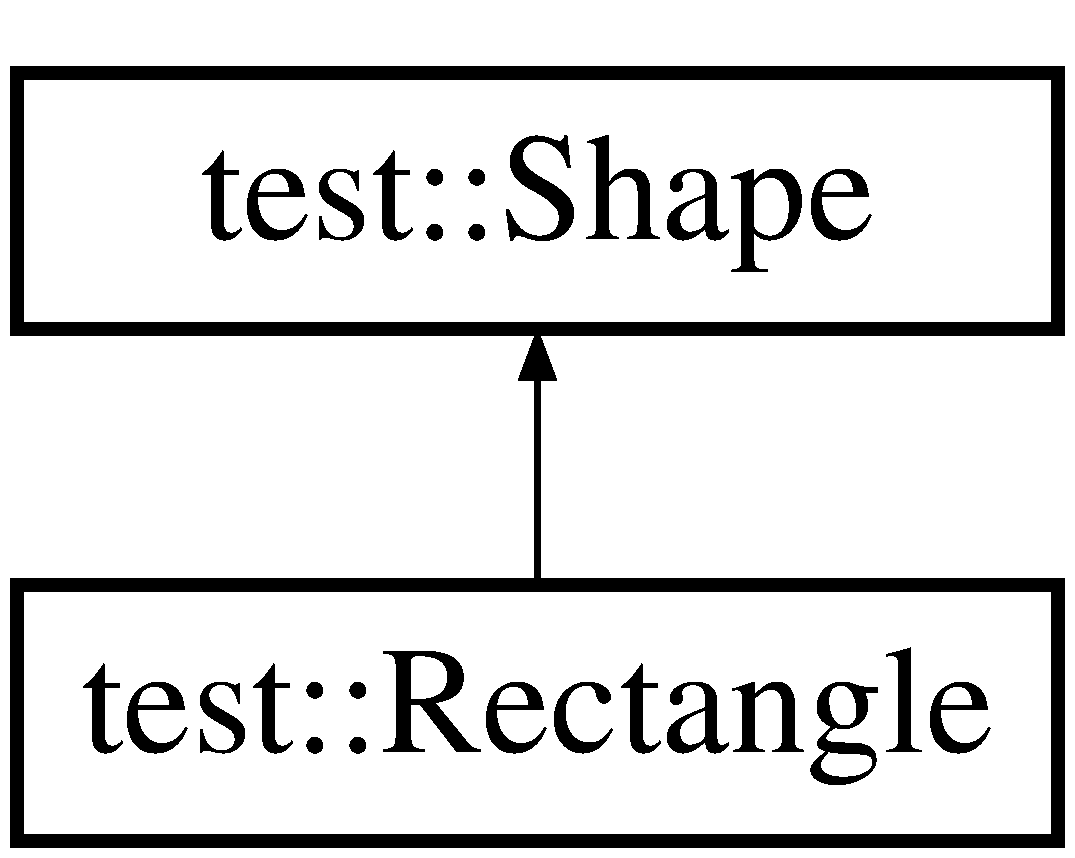
\includegraphics[height=2cm]{classtest_1_1Rectangle}
\end{center}
\end{figure}
\subsection*{Public Member Functions}
\begin{CompactItemize}
\item 
\hyperlink{classtest_1_1Rectangle_8a933e0ebd9e80ce91e61ffe87fd577e}{Rectangle} ()
\item 
\hyperlink{classtest_1_1Rectangle_494c076b13aadf26efdce07d23c61ddd}{$\sim$Rectangle} ()
\item 
virtual void \hyperlink{classtest_1_1Rectangle_22e5e5f9e3c7474d3586e1d7d36bb069}{Draw} (CDC $\ast$pDC)
\end{CompactItemize}


\subsection{Detailed Description}
\hyperlink{classtest_1_1Rectangle}{Rectangle} class define 

\subsection{Constructor \& Destructor Documentation}
\hypertarget{classtest_1_1Rectangle_8a933e0ebd9e80ce91e61ffe87fd577e}{
\index{test::Rectangle@{test::Rectangle}!Rectangle@{Rectangle}}
\index{Rectangle@{Rectangle}!test::Rectangle@{test::Rectangle}}
\subsubsection[Rectangle]{\setlength{\rightskip}{0pt plus 5cm}Rectangle::Rectangle ()}}
\label{classtest_1_1Rectangle_8a933e0ebd9e80ce91e61ffe87fd577e}


Draw fuction for this shape \begin{Desc}
\item[Parameters:]
\begin{description}
\item[{\em CDC$\ast$}]pointer to MFC CDC constructor \end{description}
\end{Desc}
\hypertarget{classtest_1_1Rectangle_494c076b13aadf26efdce07d23c61ddd}{
\index{test::Rectangle@{test::Rectangle}!$\sim$Rectangle@{$\sim$Rectangle}}
\index{$\sim$Rectangle@{$\sim$Rectangle}!test::Rectangle@{test::Rectangle}}
\subsubsection[$\sim$Rectangle]{\setlength{\rightskip}{0pt plus 5cm}Rectangle::$\sim$Rectangle ()}}
\label{classtest_1_1Rectangle_494c076b13aadf26efdce07d23c61ddd}


destructor 

\subsection{Member Function Documentation}
\hypertarget{classtest_1_1Rectangle_22e5e5f9e3c7474d3586e1d7d36bb069}{
\index{test::Rectangle@{test::Rectangle}!Draw@{Draw}}
\index{Draw@{Draw}!test::Rectangle@{test::Rectangle}}
\subsubsection[Draw]{\setlength{\rightskip}{0pt plus 5cm}void Rectangle::Draw (CDC $\ast$ {\em pDC})\hspace{0.3cm}{\tt  \mbox{[}virtual\mbox{]}}}}
\label{classtest_1_1Rectangle_22e5e5f9e3c7474d3586e1d7d36bb069}


Draw function for rectangle \begin{Desc}
\item[Parameters:]
\begin{description}
\item[{\em CDC$\ast$}]pointer to MFC CDC class \end{description}
\end{Desc}


Implements \hyperlink{classtest_1_1Shape_71718b8d8832ba737879df3d78b22204}{test::Shape}.

The documentation for this class was generated from the following files:\begin{CompactItemize}
\item 
\hyperlink{shape_8h}{shape.h}\item 
shape.cpp\end{CompactItemize}

\hypertarget{classtest_1_1Shape}{
\section{test::Shape Class Reference}
\label{classtest_1_1Shape}\index{test::Shape@{test::Shape}}
}
{\tt \#include $<$shape.h$>$}

Inheritance diagram for test::Shape::\begin{figure}[H]
\begin{center}
\leavevmode
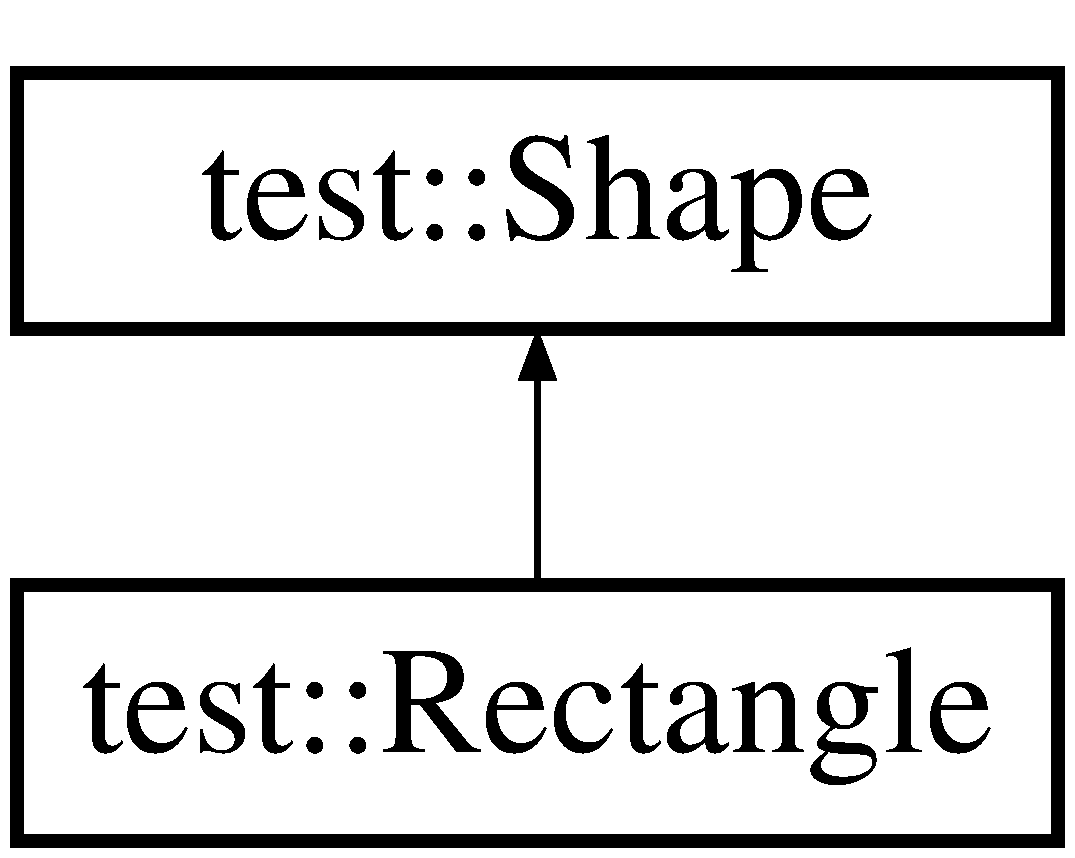
\includegraphics[height=2cm]{classtest_1_1Shape}
\end{center}
\end{figure}
\subsection*{Public Member Functions}
\begin{CompactItemize}
\item 
\hyperlink{classtest_1_1Shape_aa8d87171e65e0d8ba3c5459978992a7}{Shape} ()
\item 
\hyperlink{classtest_1_1Shape_935afc9e576015f967d90de56977167d}{$\sim$Shape} ()
\item 
virtual void \hyperlink{classtest_1_1Shape_71718b8d8832ba737879df3d78b22204}{Draw} (CDC $\ast$pDC)=0
\end{CompactItemize}


\subsection{Detailed Description}
class shape define this is the base class for all \hyperlink{classtest_1_1Shape}{Shape} 

\subsection{Constructor \& Destructor Documentation}
\hypertarget{classtest_1_1Shape_aa8d87171e65e0d8ba3c5459978992a7}{
\index{test::Shape@{test::Shape}!Shape@{Shape}}
\index{Shape@{Shape}!test::Shape@{test::Shape}}
\subsubsection[Shape]{\setlength{\rightskip}{0pt plus 5cm}Shape::Shape ()}}
\label{classtest_1_1Shape_aa8d87171e65e0d8ba3c5459978992a7}


contructor \hypertarget{classtest_1_1Shape_935afc9e576015f967d90de56977167d}{
\index{test::Shape@{test::Shape}!$\sim$Shape@{$\sim$Shape}}
\index{$\sim$Shape@{$\sim$Shape}!test::Shape@{test::Shape}}
\subsubsection[$\sim$Shape]{\setlength{\rightskip}{0pt plus 5cm}Shape::$\sim$Shape ()}}
\label{classtest_1_1Shape_935afc9e576015f967d90de56977167d}


destructor 

\subsection{Member Function Documentation}
\hypertarget{classtest_1_1Shape_71718b8d8832ba737879df3d78b22204}{
\index{test::Shape@{test::Shape}!Draw@{Draw}}
\index{Draw@{Draw}!test::Shape@{test::Shape}}
\subsubsection[Draw]{\setlength{\rightskip}{0pt plus 5cm}virtual void test::Shape::Draw (CDC $\ast$ {\em pDC})\hspace{0.3cm}{\tt  \mbox{[}pure virtual\mbox{]}}}}
\label{classtest_1_1Shape_71718b8d8832ba737879df3d78b22204}


interface 

Implemented in \hyperlink{classtest_1_1Rectangle_22e5e5f9e3c7474d3586e1d7d36bb069}{test::Rectangle}.

The documentation for this class was generated from the following files:\begin{CompactItemize}
\item 
\hyperlink{shape_8h}{shape.h}\item 
shape.cpp\end{CompactItemize}

\chapter{File Documentation}
\hypertarget{shape_8h}{
\section{shape.h File Reference}
\label{shape_8h}\index{shape.h@{shape.h}}
}
\subsection*{Namespaces}
\begin{CompactItemize}
\item 
namespace \hyperlink{namespacetest}{test}
\end{CompactItemize}
\subsection*{Classes}
\begin{CompactItemize}
\item 
class \hyperlink{classtest_1_1Shape}{test::Shape}
\item 
class \hyperlink{classtest_1_1Rectangle}{test::Rectangle}
\end{CompactItemize}


\subsection{Detailed Description}
\small\begin{alltt}{\bf Richard Zeng Shape Class File Source}\end{alltt}
\normalsize 
 \small\begin{alltt}{\bf Copyright and Use}\end{alltt}
\normalsize 


\begin{Desc}
\item[Author:]Richard Zeng \end{Desc}
\begin{Desc}
\item[Date:]2006-3-23\end{Desc}
\small\begin{alltt}\href{mailto:zengyongjoy@gmail.com}{\tt zengyongjoy@gmail.com}\end{alltt}
\normalsize 
 {\bf All rights reserved.} 
\printindex
\end{document}
